\begin{exercises}
	\begin{problist}
		\prob  Express the following lines in vector form.
		\begin{enumerate}
			\item   $\ell_1\subseteq\R^2$ with equation $4x-3y=-10$.
			\item   $\ell_2\subseteq\R^2$ which passes through the points $A=(1,1)$ and $B=(2,7)$.
			\item   $\ell_3\subseteq\R^2$ which passes through $\vec 0$ and is parallel to the line
				with equation $4x-3y=-10$.
			\item   $\ell_4\subseteq\R^3$ which passes through the points $A=(-1,-1,0)$ and $B=(2,3,5)$.
			\item   $\ell_5\subseteq\R^3$ which is contained in the $yz$-plane and where the coordinates
				of every point in $\ell_5$ satisfy $x+2y-3z=5$.
		\end{enumerate}
		\prob Express the following planes in vector form
		\begin{enumerate}
			\item   $\mathcal P_1\subseteq\R^3$ with equation $4x-z=0$.
			\item   $\mathcal P_2\subseteq\R^3$ which passes through the points $A=(-1,-1,0)$, $B=(2,3,5)$, and $C=(3,3,3)$.
			\item   $\mathcal P_3\subseteq\R^3$ with equation $4x-3y+z=-10$.
			\item   $\mathcal P_4\subseteq\R^3$ which is parallel to the $yz$-plane but passes through the point $X=(1,-1,1)$.
			\item   $\R^2$.
			\item   $\mathcal P_5\subseteq\R^4$ which passes through $A=(1,-1,1,-1)$,
				and where the coordinates of every point in $\mathcal P_5$ satisfy the equations $x+y+2z-w=3$
				and $x+y+z+w=0$.
		\end{enumerate}
		\prob Let $\ell_1$, $\ell_2$, and $\ell_3$ be described in vector form by
		\[
			\overbrace{\vec x=t\mat{1\\1}+\mat{1\\3}}^{\displaystyle \ell_1}
			\quad
			\overbrace{\vec x=t\mat{1\\3}+\mat{1\\1}}^{\displaystyle \ell_2}
			\quad
			\overbrace{\vec x=t\mat{2\\2}+\mat{2\\4}}^{\displaystyle \ell_3}.
		\]
		\begin{enumerate}
			\item
				Determine which pairs of the lines $\ell_1$, $\ell_2$, and $\ell_3$ intersect, 
				coincide, or are parallel.
			\item What is $\ell_1\cap\ell_2\cap\ell_3$?
		\end{enumerate}

		\prob Let $\mathcal P_1\subseteq\R^3$ be the plane with equation $x+2y-z=3$. Let
		$\mathcal P_2$ and $\ell$ be described in vector form by
		\[
			\overbrace{\vec x=t\mat{1\\1\\1}+s\mat{0\\0\\2}+\mat{1\\3\\1}}^{\displaystyle \mathcal P_2}
			\qquad
			\overbrace{\vec x=t\mat{1\\3\\1}+\mat{1\\1\\0}}^{\displaystyle \ell}.
		\]
		\begin{enumerate}
			\item Find $\mathcal P_1\cap \ell$.
			\item Find $\mathcal P_1\cap \mathcal P_2$.
			\item Find $\mathcal P_2\cap \ell$.
			\item Give an example of a plane $\mathcal P_3$ so that
				$\mathcal P_3\cap\ell$ is empty.
			\item Does there exist a plane $\mathcal P_2'$ that is 
				parallel to $\mathcal P_2$, but which does not
				intersect $\ell$? Why or why not?
		\end{enumerate}

	\prob
		Let $\vec a=\mat{1 \\1}$ and $\vec b=\mat{1 \\ -1}$. 
		The goal of this question is to produce a drawing of the set of convex linear combinations of $\vec a$ and $\vec b$.
		\begin{enumerate}
			\item Let $A$ be the set of all non-negative linear combinations of $\vec a$ and $\vec b$. Draw $A$.
			\item Let $\ell$ be the set 
			\[
				\Set{\alpha \vec a + \beta \vec b\given \alpha, \beta \in \R\text{ and } \alpha+\beta = 1}
			\]
			Rewrite $\ell$ in set-builder notation using only a single variable $t$. (Hint: Let $t$ be $\alpha$.)
			\item Justify why $\ell$ is a line, and write $\ell$ in vector form.
			\item Draw both $A$ and $\ell$ on the same grid. On a separate grid, draw $A\cap \ell$.
			\item	Write the $A \cap \ell$ in set builder notation. 
				How does $A\cap \ell$ relate to convex linear combinations?
			\item Determine the endpoints of $A \cap \ell$.
		\end{enumerate}
		\begin{solution}
			\begin{enumerate}
				\item 
				\begin{tikzpicture}[baseline = (current bounding box.north)]
					\begin{axis}[
						anchor=origin,
						disabledatascaling,
						xmin=-1,xmax=2,
						ymin=-1,ymax=1,
						xtick={-2,...,3},
						ytick={-2,...,3},
						x=1cm,y=1cm,
						grid=both,
						grid style={line width=.1pt, draw=gray!10},
						%major grid style={line width=.2pt,draw=gray!50},
						axis lines=middle,
						minor tick num=0,
						enlargelimits={abs=0.5},
						axis line style={latex-latex},
						ticklabel style={font=\tiny,fill=white},
						xlabel style={at={(ticklabel* cs:1)},anchor=north west},
						ylabel style={at={(ticklabel* cs:1)},anchor=south west}
					]
						\fill [mygreen, opacity=.3] (0,0) -- (3,3) -- (3,-3) -- cycle;
						\draw [black, thick, dashed, ->] (0,0) -- (1,1) node[midway, above left] {$\vec a$};
						\draw [black, thick, dashed, ->] (0,0) -- (1,-1) node[midway, below left, yshift=2pt] {$\vec b$};
					\end{axis}
					\node[mygreen] at (1.5,0.25) {$A$};
				\end{tikzpicture}
				\item $\ell$
				is given by the set
				\[
					\Set{\vec x\in\R^2\given \vec x=t \vec a + (1-t) \vec b\text{ for some }t\in\R}.
				\]
				 \item The above set can be rewritten as
				\[
					\Set{\vec x\in\R^2\given \vec x=t (\vec a - \vec b)+\vec b\text{ for some }t\in\R}.
				\]
				 This is exactly the line given in vector form by
				\[
					\vec x = t(\vec a - \vec b)+\vec b.
				\]
				Since $\vec a-\vec b=\mat{0\\2}$, 
				$\ell$ is the vertical line containing $\vec b$ (and $\vec a$).

				\item 
				\begin{tikzpicture}[baseline = (current bounding box.north)]
					\begin{axis}[
						anchor=origin,
						disabledatascaling,
						xmin=-1,xmax=2,
						ymin=-1,ymax=1,
						xtick={-2,...,3},
						ytick={-2,...,3},
						x=1cm,y=1cm,
						grid=both,
						grid style={line width=.1pt, draw=gray!10},
						%major grid style={line width=.2pt,draw=gray!50},
						axis lines=middle,
						minor tick num=0,
						enlargelimits={abs=0.5},
						axis line style={latex-latex},
						ticklabel style={font=\tiny,fill=white},
						xlabel style={at={(ticklabel* cs:1)},anchor=north west},
						ylabel style={at={(ticklabel* cs:1)},anchor=south west}
					]
						\fill [mygreen, opacity=.3] (0,0) -- (3,3) -- (3,-3) -- cycle;
						\draw [black, thick, dashed, ->] (0,0) -- (1,1) node[midway, above left] {$\vec a$};
						\draw [black, thick, dashed, ->] (0,0) -- (1,-1) node[midway, below left, yshift=2pt] {$\vec b$};
						\draw [WildStrawberry, thick, -] (1,2) -- (1,-2);
					\end{axis}
					\node[WildStrawberry] at (0.75,-1.25) {$\ell$};
					\node[mygreen] at (1.5,0.25) {$A$};
				\end{tikzpicture}
				
				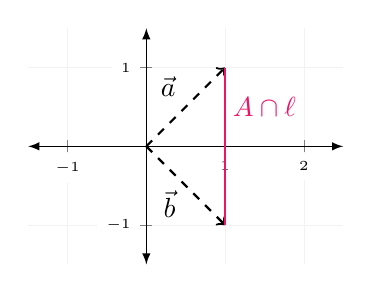
\begin{tikzpicture}[baseline = (current bounding box.north)]
					\begin{axis}[
						anchor=origin,
						disabledatascaling,
						xmin=-1,xmax=2,
						ymin=-1,ymax=1,
						xtick={-2,...,3},
						ytick={-2,...,3},
						x=1cm,y=1cm,
						grid=both,
						grid style={line width=.1pt, draw=gray!10},
						%major grid style={line width=.2pt,draw=gray!50},
						axis lines=middle,
						minor tick num=0,
						enlargelimits={abs=0.5},
						axis line style={latex-latex},
						ticklabel style={font=\tiny,fill=white},
						xlabel style={at={(ticklabel* cs:1)},anchor=north west},
						ylabel style={at={(ticklabel* cs:1)},anchor=south west}
					]
						\draw [black, thick, dashed, ->] (0,0) -- (1,1) node[midway, above left] {$\vec a$};
						\draw [black, thick, dashed, ->] (0,0) -- (1,-1) node[midway, below left, yshift=2pt] {$\vec b$};
						\draw [WildStrawberry, thick, -] (1,1) -- (1,-1);
					\end{axis}
					\node[WildStrawberry] at (1.5,0.5) {$A \cap \ell$};
				\end{tikzpicture}
				
				\item $A \cap \ell$ is the set
				\[
					\Set{\alpha \vec a+\beta \vec b\given \alpha,\beta \geq 0\text{ and }
					\alpha+\beta = 1}.
				\]
				This is the set of convex linear
				combinations of $\vec a$ and $\vec b$. 
				\item $A
				\cap \ell$ is the line segment with endpoints $\vec a$ and $\vec b$.
			\end{enumerate}
		\end{solution}

	\prob
		Let $\vec a=\mat{2 \\0}$, $\vec b=\mat{0 \\ 2}$, and $\vec c=\mat{-1 \\ -1}$. 
		The goal of this question is to produce a drawing of the set of 
		convex linear combinations of $\vec a$, $\vec b$, and $\vec c$. This requires an understanding of the previous question.
		\begin{enumerate}
		\item \label{PROBaconvex} Let $\vec d=\mat{1 \\ 1}$. Write $\vec d$ as a convex
			linear combination of $\vec a$ and $\vec b$.
		\item \label{PROBbconvex} Let $\vec e=\mat{0 \\ 0}$. Write $\vec e$ as a convex 
			linear combination of $\vec c$ and $\vec d$.
		\item Substituting the answer to (\ref{PROBaconvex}) into the answer to part
			(\ref{PROBbconvex}), write $\vec e$ as a convex linear combination of $\vec a$, $\vec b$, and $\vec c$.
		\item Draw and label $\vec a$, $\vec b$, $\vec c$, $\vec d$, and
			$\vec e$ on the same grid.
		\item Draw the set of convex linear combinations of $\vec a$, $\vec b$, 
			and $\vec c$. Justify your answer.
		\end{enumerate}
	\begin{solution}
		\begin{enumerate}
			\item
			$
				\vec d = \tfrac{1}{2}\vec a + \tfrac{1}{2}\vec b.
			$
			\item
			$
				\vec e= \tfrac{1}{2}\vec c+\tfrac{1}{2}\vec d.
			$
			\item
			\begin{align*}
				\vec e & = \tfrac{1}{2}\vec c+\tfrac{1}{2}(\tfrac{1}{2}\vec a + \tfrac{1}{2}\vec b)\\
				       & = \tfrac{1}{2}\vec c+\tfrac{1}{4}\vec a + \tfrac{1}{4}\vec b.
			\end{align*}
			\item 
			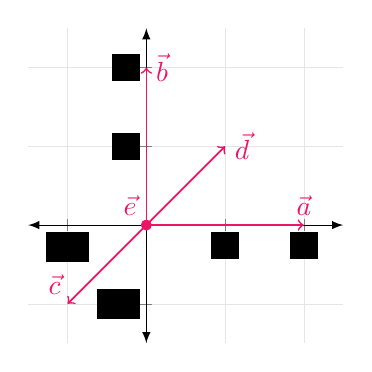
\begin{tikzpicture}[baseline = (current bounding box.north)]
				\begin{axis}[
					anchor=origin,
					name=plot1,
					disabledatascaling,
					xmin=-1,xmax=2,
					ymin=-1,ymax=2,
					xtick={-4,...,4},
					ytick={-2,...,4},
					x=1cm,y=1cm,
					grid=both,
					grid style={line width=.1pt, draw=black!10},
					%major grid style={line width=.2pt,draw=gray!50},
					axis lines=middle,
					minor tick num=0,
					enlargelimits={abs=0.5},
					axis line style={latex-latex},
					ticklabel style={font=\tiny,fill=\currentbackgroundcolor},
					xlabel style={at={(ticklabel* cs:1)},anchor=north west},
					ylabel style={at={(ticklabel* cs:1)},anchor=south west}
				]
					\coordinate (A) at (2,0);
					\coordinate (B) at (0,2);
					\coordinate (C) at (-1,-1);
					\coordinate (D) at (1,1);
					\coordinate (E) at (0,0);
					\fill[WildStrawberry] (E) circle (2pt) node[above left] {$\vec e$};
					\draw[semithick, WildStrawberry, ->] (0,0) -- (A);
					\draw[semithick, WildStrawberry, ->] (0,0) -- (B);
					\draw[semithick, WildStrawberry, ->] (0,0) -- (C);
					\draw[semithick, WildStrawberry, ->] (0,0) -- (D);
				\end{axis}
				\node[above, WildStrawberry] at (A) {$\vec a$};
				\node[right, WildStrawberry] at (B) {$\vec b$};
				\node[above left, WildStrawberry, xshift=1pt] at (C) {$\vec c$};
				\node[right, WildStrawberry] at (D) {$\vec d$};
			\end{tikzpicture}
			\item 
			\begin{tikzpicture}[baseline = (current bounding box.north)]
				\begin{axis}[
					anchor=origin,
					name=plot1,
					disabledatascaling,
					xmin=-1,xmax=2,
					ymin=-1,ymax=2,
					xtick={-4,...,4},
					ytick={-2,...,4},
					x=1cm,y=1cm,
					grid=both,
					grid style={line width=.1pt, draw=black!10},
					%major grid style={line width=.2pt,draw=gray!50},
					axis lines=middle,
					minor tick num=0,
					enlargelimits={abs=0.5},
					axis line style={latex-latex},
					ticklabel style={font=\tiny,fill=\currentbackgroundcolor},
					xlabel style={at={(ticklabel* cs:1)},anchor=north west},
					ylabel style={at={(ticklabel* cs:1)},anchor=south west}
				]
					\coordinate (A) at (2,0);
					\coordinate (B) at (0,2);
					\coordinate (C) at (-1,-1);
					\fill[mygreen, opacity=.3] (A) -- (B) -- (C) -- cycle;
					\fill [black] (A) circle (2pt) node [above, yshift=1pt] {$\vec a$};
					\fill [black] (B) circle (2pt) node [above right] {$\vec b$};
					\fill [black] (C) circle (2pt) node [above left, xshift=1pt] {$\vec c$};
				\end{axis}
			\end{tikzpicture}
			
			The set is the filled-in
			triangle with vertices given by $\vec a$,
			$\vec b$, and $\vec c$. To see this, notice
			that the set of convex linear combinations of
			$\vec a$, $\vec b$, and $\vec c$ is the set of
			convex linear combinations of $\vec c$ and any
			convex linear combination of $\vec a$ and
			$\vec b$. Indeed,
			\[
			\begin{split}
				&\alpha_{1} \vec a+\alpha_{2} \vec b+ \alpha_{3}
				\vec c \\
				&\qquad= (1-\alpha_{3})\left(\tfrac{\alpha_1}{1-\alpha_3}\vec
				a + \tfrac{\alpha_2}{1-\alpha_3}\vec b\right)+\alpha_{3}
				\vec c,
			\end{split}
			\]
			and $\alpha_{1} \vec a+\alpha_{2} \vec b+ \alpha_{3}
			\vec c$ is a convex linear combination of $\vec
			a$, $\vec b$, and $\vec c$ exactly when
			\[
				\frac{\alpha_1}{1-\alpha_3}\vec a + \frac{\alpha_2}{1-\alpha_3}\vec b
			\]
			 is a convex linear combination of $\vec a$ and $\vec
			b$ (verify this!).
				By the previous part, the set of convex linear combinations
			of $\vec a$ and $\vec b$ is the line segment
			between $\vec a$ and $\vec b$. Call this line segment $S$.
			Now we know the set of convex linear
			combinations of $\vec a$, $\vec b$, and $\vec c$
			is the union of every line segment from $\vec c$
			and a vector in $S$. This is the solid triangle with
			vertices given by $\vec a$, $\vec b$, and $\vec	c$.
		\end{enumerate}
	\end{solution}

	\prob
		Let $\vec x=\mat{1 \\ 1}$, $\vec y = \mat{3 \\ -1}$ and $\vec z=\mat{-2 \\ -2}.$  Draw the following subsets of $\R^2$.
		\begin{enumerate}
		\item All non-negative linear combinations of $\vec x$ and $\vec y$.
		\item All non-negative linear combinations of $\vec x$ and $\vec z$.
		\item\label{PROBcconvex} All convex linear combinations of $\vec y$ and $\vec z$.
		\item\label{PROBdconvex} All convex linear combinations of $\vec x$ and $\vec z$.
		\item All convex linear combinations of $\vec x$, $\vec y$ and $\vec z$.

		\end{enumerate}
	\begin{solution}
		\begin{enumerate}
			\item 
			\begin{tikzpicture}[baseline = (current bounding box.north)]
				\begin{axis}[
					anchor=origin,
					disabledatascaling,
					xmin=0,xmax=3,
					ymin=-1,ymax=1,
					xtick={-2,...,3},
					ytick={-2,...,3},
					x=1cm,y=1cm,
					grid=both,
					grid style={line width=.1pt, draw=gray!10},
					%major grid style={line width=.2pt,draw=gray!50},
					axis lines=middle,
					minor tick num=0,
					enlargelimits={abs=0.5},
					axis line style={latex-latex},
					ticklabel style={font=\tiny,fill=white},
					xlabel style={at={(ticklabel* cs:1)},anchor=north west},
					ylabel style={at={(ticklabel* cs:1)},anchor=south west}
				]
					\fill [mygreen, opacity=.3] (0,0) -- (5,5) -- (5,-5/3) -- cycle;
					\draw [black, thick, dashed, ->] (0,0) -- (1,1) node[midway, above left] {$\vec x$};
					\draw [black, thick, dashed, ->] (0,0) -- (3,-1) node[midway, below left, yshift=2pt] {$\vec y$};
				\end{axis}
			\end{tikzpicture}
			\item 
			\begin{tikzpicture}[baseline = (current bounding box.north)]
				\begin{axis}[
					anchor=origin,
					disabledatascaling,
					xmin=-2,xmax=1,
					ymin=-2,ymax=1,
					xtick={-2,...,3},
					ytick={-2,...,3},
					x=1cm,y=1cm,
					grid=both,
					grid style={line width=.1pt, draw=gray!10},
					%major grid style={line width=.2pt,draw=gray!50},
					axis lines=middle,
					minor tick num=0,
					enlargelimits={abs=0.5},
					axis line style={latex-latex},
					ticklabel style={font=\tiny,fill=white},
					xlabel style={at={(ticklabel* cs:1)},anchor=north west},
					ylabel style={at={(ticklabel* cs:1)},anchor=south west}
				]
					\fill [black] (1,1) circle (2pt) node [below right] {$\vec x$};
					\fill [black] (-2,-2) circle (2pt) node [below right] {$\vec z$};
					\draw [mygreen, thick, -] (2,2) -- (-3,-3);
				\end{axis}
			\end{tikzpicture}
			\item 
			\begin{tikzpicture}[baseline = (current bounding box.north)]
				\begin{axis}[
					anchor=origin,
					disabledatascaling,
					xmin=-2,xmax=3,
					ymin=-2,ymax=0,
					xtick={-2,...,3},
					ytick={-2,...,3},
					x=1cm,y=1cm,
					grid=both,
					grid style={line width=.1pt, draw=gray!10},
					%major grid style={line width=.2pt,draw=gray!50},
					axis lines=middle,
					minor tick num=0,
					enlargelimits={abs=0.5},
					axis line style={latex-latex},
					ticklabel style={font=\tiny,fill=white},
					xlabel style={at={(ticklabel* cs:1)},anchor=north west},
					ylabel style={at={(ticklabel* cs:1)},anchor=south west}
				]
					\fill [black] (3,-1) circle (2pt) node [below right] {$\vec y$};
					\fill [black] (-2,-2) circle (2pt) node [below right] {$\vec z$};
					\draw [mygreen, thick, -] (3,-1) -- (-2,-2);
				\end{axis}
			\end{tikzpicture}
			\item 
			\begin{tikzpicture}[baseline = (current bounding box.north)]
				\begin{axis}[
					anchor=origin,
					disabledatascaling,
					xmin=-2,xmax=1,
					ymin=-2,ymax=1,
					xtick={-2,...,3},
					ytick={-2,...,3},
					x=1cm,y=1cm,
					grid=both,
					grid style={line width=.1pt, draw=gray!10},
					%major grid style={line width=.2pt,draw=gray!50},
					axis lines=middle,
					minor tick num=0,
					enlargelimits={abs=0.5},
					axis line style={latex-latex},
					ticklabel style={font=\tiny,fill=white},
					xlabel style={at={(ticklabel* cs:1)},anchor=north west},
					ylabel style={at={(ticklabel* cs:1)},anchor=south west}
				]
					\fill [black] (1,1) circle (2pt) node [below right] {$\vec x$};
					\fill [black] (-2,-2) circle (2pt) node [below right] {$\vec z$};
					\draw [mygreen, thick, -] (1,1) -- (-2,-2);
				\end{axis}
			\end{tikzpicture}
			\item
			\begin{tikzpicture}[baseline = (current bounding box.north)]
				\begin{axis}[
					anchor=origin,
					disabledatascaling,
					xmin=-2,xmax=3,
					ymin=-2,ymax=1,
					xtick={-2,...,3},
					ytick={-2,...,3},
					x=1cm,y=1cm,
					grid=both,
					grid style={line width=.1pt, draw=gray!10},
					%major grid style={line width=.2pt,draw=gray!50},
					axis lines=middle,
					minor tick num=0,
					enlargelimits={abs=0.5},
					axis line style={latex-latex},
					ticklabel style={font=\tiny,fill=white},
					xlabel style={at={(ticklabel* cs:1)},anchor=north west},
					ylabel style={at={(ticklabel* cs:1)},anchor=south west}
				]
					\fill [mygreen, opacity=.3] (1,1) -- (3,-1) -- (-2,-2) -- cycle;
					\fill [black] (1,1) circle (2pt) node [left, yshift=1pt] {$\vec x$};
					\fill [black] (3,-1) circle (2pt) node [below right] {$\vec y$};
					\fill [black] (-2,-2) circle (2pt) node [below right] {$\vec z$};
				\end{axis}
			\end{tikzpicture}
		\end{enumerate}
	\end{solution}

	\prob Describe the sets in (\ref{PROBcconvex}) and (\ref{PROBdconvex}) in set builder notation.
	\begin{solution}
		(\ref{PROBcconvex}) 
		\[
			\Set*{\vec v \in \R^{2}\given \vec v=t\mat{-5\\-1}+\mat{3\\-1}\text{ for some }0\leq t\leq 1}.
		\]
		
		(\ref{PROBdconvex}) 
		\[
			\Set*{\vec w \in \R^{2}\given \vec w=t\mat{-3\\-3}+\mat{1\\1}\text{ for some }0\leq t\leq 1}.
		\]
	\end{solution}

	\prob
		Determine if the points $P=(-2,0)$ and $Q=(0,-2)$ are convex linear 
		combinations of the vectors $\vec u =\mat{1 \\4}$, $\vec v =\mat{-5 \\8}$, 
		and $\vec w =\mat{-2 \\-6}$. First solve this question by drawing a picture. Then justify algebraically.
	\begin{solution}
		\begin{tikzpicture}[baseline = (current bounding box.north)]
			\begin{axis}[
				anchor=origin,
				disabledatascaling,
				xmin=-5,xmax=1,
				ymin=-6,ymax=8,
				xtick={-5,...,1},
				ytick={-6,-4,-2,0,2,4,6,8},
				x=1cm,y=0.5cm,
				grid=both,
				grid style={line width=.1pt, draw=gray!10},
				%major grid style={line width=.2pt,draw=gray!50},
				axis lines=middle,
				minor tick num=0,
				enlargelimits={abs=0.5},
				axis line style={latex-latex},
				ticklabel style={font=\tiny,fill=white},
				xlabel style={at={(ticklabel* cs:1)},anchor=north west},
				ylabel style={at={(ticklabel* cs:1)},anchor=south west}
			]
				\coordinate (P) at (-2,0);
				\coordinate (Q) at (0,-2);
				\coordinate (U) at (1,4);
				\coordinate (V) at (-5,8);
				\coordinate (W) at (-2,-6);
				\fill [mygreen, opacity=.3] (U) -- (V) -- (W) -- cycle;
				\fill [mypink] (P) circle (2pt) node [above, yshift=1pt] {$P$};
				\fill [mypink] (Q) circle (2pt) node [right, xshift=1pt] {$Q$};
				\fill [black] (U) circle (2pt) node [above, yshift=1pt] {$\vec u$};
				\fill [black] (V) circle (2pt) node [below left] {$\vec v$};
				\fill [black] (W) circle (2pt) node [left, xshift=-1pt] {$\vec w$};
			\end{axis}
		\end{tikzpicture}
		
		Geometrically, the set of convex linear combinations of $\vec u$, $\vec v$, and $\vec w$ is a
		filled-in triangle with vertices at $\vec u, \vec v$ and $\vec w$. The point
		$P$ lies inside this triangle, while $Q$ does not.
		
		To argue algebraically, suppose 
		$P=t_{1}\vec u + t_{2}\vec v + t_{3} \vec w$ and
		$t_{1}+t_{2}+t_{3}=1$. From these assumptions, we can set up a system of equations
		which has a unique solution
		\[
			P=\tfrac14 \vec u + \tfrac14 \vec v + \tfrac12 \vec w,
		\]
		and so $P$ is a convex linear combination of $\vec u$, $\vec v$, and $\vec w$.
		 The same procedure with $Q$ gives a unique solution with coefficients
		$t_{1}=\frac 59, t_{2}=-\frac 19, t_{3}=\frac 59$, and so $Q$ is
		not a convex linear combination of $\vec u$, $\vec v$, and $\vec w$.
	\end{solution}
	\end{problist}
\end{exercises}
